\documentclass[14pt]{article}
\usepackage[left=0.5in, right=.5in, top=0.5in, bottom=0.75in]{geometry}
\usepackage{enumitem}
\usepackage{amsmath}
\usepackage{bbold}

\usepackage[left=0.5in, right=.5in, top=0.5in, bottom=0.75in]{geometry}
\usepackage{hyperref}
\usepackage{subfig}
\usepackage{graphicx}
\usepackage{caption}
\hypersetup{colorlinks,linkcolor={blue},citecolor={blue}, urlcolor={red}}
\begin{document}
	\title{Lab works : Subject 1}
	\date{}
\author{\textbf{Mahmoud El Omar}}

\maketitle
\pagenumbering{arabic}
\section*{Theoretical Study in the case of sine wave}
We have the following signal :
\begin{align*}
	x(t) = a\cos(2\pi f_0t + \phi) 
\end{align*}
	\begin{enumerate}[label=\alph*)]
	 \item We already know that $\mathcal{F}_{cc}\{\cos(2\pi f_0t)\} = \frac{1}{2}(\delta (f-f_0) + \delta(f+f_0))$ and $\mathcal{F}_{cc}\{\sin(2\pi f_0t)\} = \frac{1}{2j}(\delta (f-f_0) - \delta(f+f_0))$ \break
	\newline
	 $x(t) = a\cos(2\pi f_0t + \phi) = a(\cos(2\pi f_0t)\cos(\phi) - \sin(2\pi f_0t)\sin(\phi)) \Rightarrow \newline 
	 \newline $For the sake of notation simplicity, let's denote $ \boxed{X(f) =  \mathcal{F}_{cc}x(f)}$ and $\boxed{X_s(\lambda) = \mathcal{F}_{dc}x_s(\lambda)}$ \newline \newline
	 \begin{equation*}
	 	X(f) = \frac{a}{2}\cos(\phi)(\delta (f-f_0) + \delta(f+f_0)) + \frac{a}{2j}\sin(\phi)(\delta (f-f_0) - \delta(f+f_0)) \Rightarrow \newline \newline
	  \boxed{X(f) = \frac{a}{2}(\delta(f-f_0)e^{j\phi} + \delta(f+f_0)e^{-j\phi})}
	 \end{equation*}

	  \item The sampled signal  $x_s[n] = x(nT_s) = x(\frac{n}{f_s}) = a\cos(2\pi \frac{f_0}{f_s}n + \phi) = a\cos(2\pi \lambda_0 n + \phi)$ with $\lambda_0 = \frac{f_0}{f_s}$
	  \begin{equation*}
	  	X_s(\lambda) = \sum_{n=-\infty}^{\infty} x_s[n]e^{-j2\pi \lambda n} = \sum_{n=-\infty}^{\infty} a\cos(2\pi \lambda_0 n+ \phi)e^{-j2\pi \lambda n}
	 \end{equation*}
	 
	 \begin{equation*}
	 X_s(\lambda) = \frac{a}{2}\sum_{n=-\infty}^{\infty}e^{j2\pi \lambda_0 n}e^{-j2\pi \lambda n}e^{j\phi} + e^{-j2\pi \lambda_0 n}e^{-j2\pi \lambda n}e^{-j\phi}
	 \end{equation*}
	
	\begin{align*}
		X_s(\lambda) = e^{j\phi}\frac{a}{2}\sum_{n=-\infty}^{\infty}e^{-j2\pi (\lambda - \lambda_0) n} + \sum_{n=-\infty}^{\infty}e^{-j2\pi (\lambda + \lambda_0) n}
 	\end{align*}
 	\begin{equation*}
 	\boxed{
 		X_s(\lambda) = \frac{a}{2}e^{j\phi}\sum_{k = -\infty}^{\infty}\delta(\lambda - \lambda_0 - k) +\frac{a}{2}e^{-j\phi}\sum_{k = -\infty}^{\infty}\delta(\lambda + \lambda_0 - k)}
 	\end{equation*}
Using the scaling property of the Dirac delta function : $|a|\delta(at) = \delta(t)$, and since $\lambda = \frac{f}{f_s}$ and $\lambda_0 = \frac{f_0}{f_s}$, we can reach the following : 
	\begin{equation*}
		\mathcal{F}_{dc}x_s(\lambda) = \mathcal{F}_{dc}x_s(\frac{f}{f_s}) = \frac{a}{2}e^{j\phi}\sum_{k = -\infty}^{\infty}\delta(\frac{f-f_0 - kf_s}{f_s}) +  \frac{a}{2}e^{-j\phi}\sum_{k = -\infty}^{\infty}\delta{\frac{f+f_0 - kf_s}{f_s})}
	\end{equation*}
	\begin{equation*}
		\mathcal{F}_{dc}x_s(\frac{f}{f_s}) =  \frac{af_s}{2}e^{j\phi}\sum_{k = -\infty}^{\infty}\delta(f-f_0 - kf_s) +  \frac{af_s}{2}e^{-j\phi}\sum_{k = -\infty}^{\infty}\delta(f+f_0 - kf_s)
	\end{equation*}	

	\begin{equation*}
		\boxed{\frac{1}{f_s}\mathcal{F}_{dc}x_s(\frac{f}{f_s}) =  \frac{a}{2}e^{j\phi}\sum_{k = -\infty}^{\infty}\delta(f-f_0 - kf_s) +  \frac{af_s}{2}e^{-j\phi}\sum_{k = -\infty}^{\infty}\delta(f+f_0 - kf_s)}
	\end{equation*}

	\item The Fourier Transform of rect${_N{_t}}$ is the Dirichlet kernel $D_{N_{t}}(\lambda)$ as defined in the course notes.
	\begin{equation*}
	y[n] = x_s[n]\text{rect}_{N_t} \iff Y(\lambda) = X_s(\lambda)*D_{N_{t}}(\lambda)
	\end{equation*}
	\begin{equation*}
	\boxed{Y(\lambda) = \frac{a}{2}e^{j\phi}\sum_{k = -\infty}^{\infty}D_{N_{t}}(\lambda - \lambda_0 - k) +\frac{a}{2}e^{-j\phi}\sum_{k = -\infty}^{\infty}D_{N_{t}}(\lambda + \lambda_0 - k)}
	\end{equation*}
	\newpage
	\item Since $f_s >>2f_0$, therefore the Shannon condition is satisfied and the periodic spectrums do not overlap, we can perform all our calculations on just one period of the spectrum $Y(\lambda)$ without loss of generalisation. We can chose any portion of the spectrum that is equal to 1 \textit{(since $Y(\lambda)$ is 1-periodic)}. So for reasons of symmetry, I will chose the period centred around 0, that corresponds to $k=0$ in the previous equation.
	\newline \newline
	From here on out, I will consider that : 
	\begin{equation*}
	Y(\lambda) = \frac{a}{2}e^{j\phi}D_{N_t}(\lambda - \lambda_0) + \frac{a}{2}e^{-j\phi}D_{N_t}(\lambda + \lambda_0)
	\end{equation*}
	To sample $Y(\lambda)$, we need to take its value at frequencies multiple of $\frac{1}{N_f}$, so if we multiply $Y(\lambda)$ with a discrete comb of repeated deltas with period equal to $\frac{1}{N_f}$. In other words, replace $\lambda$ with $\frac{n}{N_f} \text{where} n \in \mathbb{Z}$ in $Y(\lambda)$ and we will manage to get the desired sampled spectrum : 
	\begin{equation*}
	Y_{N_f}[n] = Y(\lambda)\textbf{1}_{\uparrow N_f}[n] = 	Y(\lambda)\sum_{k = -\infty}^{\infty}\delta[n - \frac{k}{N_f}]	 = Y(\frac{k}{N_f})
	\end{equation*}
	\begin{equation*}
		Y_{N_f}[n] = \frac{a}{2}e^{j\phi}D_{N_t}(\frac{n - n_0}{N_f}) + \frac{a}{2}e^{-j\phi}D_{N_t}(\frac{n + n_0}{N_f})
	\end{equation*}
	\begin{figure}[hp]
		\centering		
		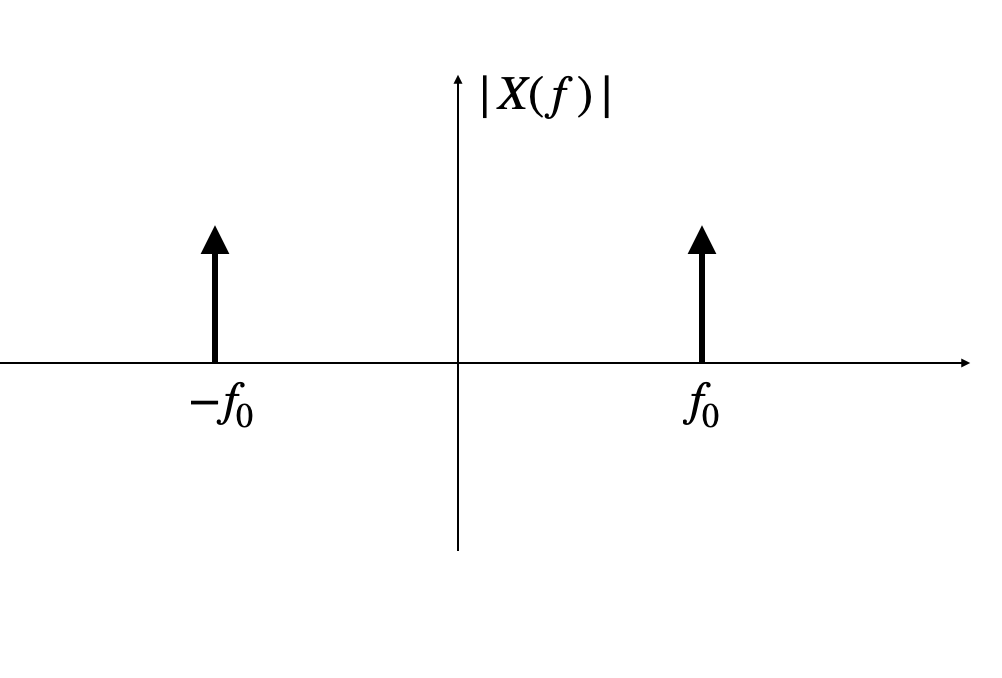
\includegraphics[width = 10cm]{1}
		\caption{Plot of the Spectrum of $x(t)$.}
		\label{fig1}
	\end{figure}
	\begin{figure}[hp]
		\centering		
		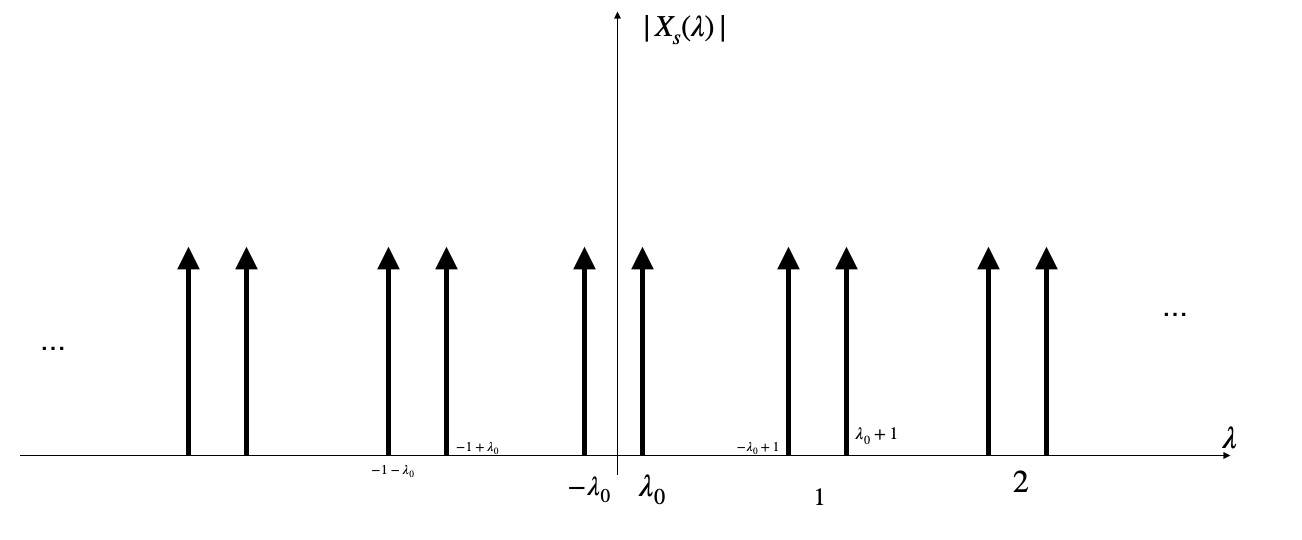
\includegraphics[width = 16cm]{3.png}
		\caption{Plot of the Spectrum of $x_s[n]$.}
		\label{fig2}
	\end{figure}
	
	\begin{figure}[t]
		\centering		
		\includegraphics[width = 20cm]{2.jpg}
		\caption{Plot of the Spectrum of $y[n]$ over 2 periods.}
		\label{fig1}
	\end{figure}

	\end{enumerate}
	\section*{Numerical Implementation}
	\begin{enumerate}[label=\alph*)]
	\item If $N_f$ = $N_t$, we can recognise the formula for the Discrete Fourier Transform, where the result of this computation is the discrete spectrum of the discrete time signal $y[n]$, and it allows us to obtain the spectral samples directly from the time samples.
	\item If $N_f \geq N_t$, then we can zero samples after the $N_t -1 $ sample of the original signal until we can have $N_f = N_t$ and then, we'll be able to calculate the Discrete Fourier Transform and obtain the spectral samples.
	\end{enumerate}	
	
\end{document}
w